\subsection{ResNet}\label{resultsReNet}

\subsubsubsection{Setup and reproducibility:}\label{setup}
All ResNet models presented here were trained on the same PC using Windows 11, Python 3.10.11 and an Nvidia RTX4090 graphics card. In order to ensure a consistent split for training and test data, the random seeds for numpy and torch were set to 22. No such steps were taken to make the training itself, using cuda, more reproducible, leading to small but noticeable variations in the results between different training runs using the same parameters.

\subsubsubsection{Hyperparameters:}\label{Hyperparameters}
In the first stages of our experimentation, we tried to identify the best hyperparameters by making multiple test runs using ResNet18 and identifying the best performances. With this approach, we aimed to get a better understanding of the impact different parameters have, before starting to use larger models that take significantly more time to train. All of our tests here used the previously discussed data augmentation. As mentioned before, multiple training cycles with the same parameters would lead to marginally different results, and in very few extreme cases, even to an accuracy difference of up to 2\%. Due to this, some of the following results might not be representative, especially if the margin between two parameters is very small. All Training was done with enabeled dataset balancing and data-augmentation allready discussed To decide on the optimizer, we compared three different ones: Adagrad, Adam, NAdam and SGD\@. Prior to this, our expectation was, that Adam would be the optimal choice and that SGD would perform the worst. Our test results (worst to best) were the following: SGD with an average loss = 0.08, followed by NAdam and Adam both having an average loss = 0.06, and finally Adagrad with an average loss of 0.035. Based on this we chose Adagrad for our further training. For our learning rate, we used an adaptive learning rate scheduler for most of the later training. Despite Adagrad inherently adjusting the learning rate, we still found that the results using a learning rate scheduler were either better over many epochs or, at worst, made no difference. In these early stages, we found that an optimal starting learning rate was somwhere between 0.001 and 0.0001. After implementing the learning rate scheduler, we defaulted to a starting learning rate of 0.0005. For our Training and validation split, we chose 80/20. Here we did not do any testing, as the number seemed adequate for the size of the dataset. The batch size did not have any noticeable impact on the performance of the model. We ended up using a batch size of 64 for all the training, as it proved to be more practical with the larger models. Changing it to 100, for example, would lead to a ResNet152 using more than 21 GB of Video RAM\@. To prevent overfitting but still have the option to train our models until they converge, we implemented an early stopping criterion. Here, the new best model would be saved each time it improved based on validation accuracy and then stop training after a set number of epochs without improvement. As we wanted to make sure our models had converged, the maximum number of epochs for our final models was set to 200 and the early stopping patience to 20 epochs. For the normalization of the images, we calculated the mean and standard deviation of the whole dataset and normalized it based on these results. Below, in table~\ref{tab:hyperparameters}, you can see our final hyperparameters. 

\begin{table}[h]
\centering
\begin{tabular}{ll}
\hline
\textbf{Hyper-Parameter} & \textbf{Value} \\
\hline
Learning rate & 0.0005 \\
Batch size & 64 \\
Split & 80/20 \\
Optimizer & Adagrad \\
Max epochs & 200 \\
\hline
\end{tabular}
\caption{Overview of Hyperparameters}~\label{tab:hyperparameters}
\end{table} 


\subsubsubsection{ResNet18:}\label{ResNet18}
Training ResNet18 with our optimized hyperparameters already gave us great results. Our very first attempts, without any optimisations lead to an validation accuracy of about 97\% as seen in figure\ref{fig:resNet18first}.
\begin{figure}[ht]
    \centering
    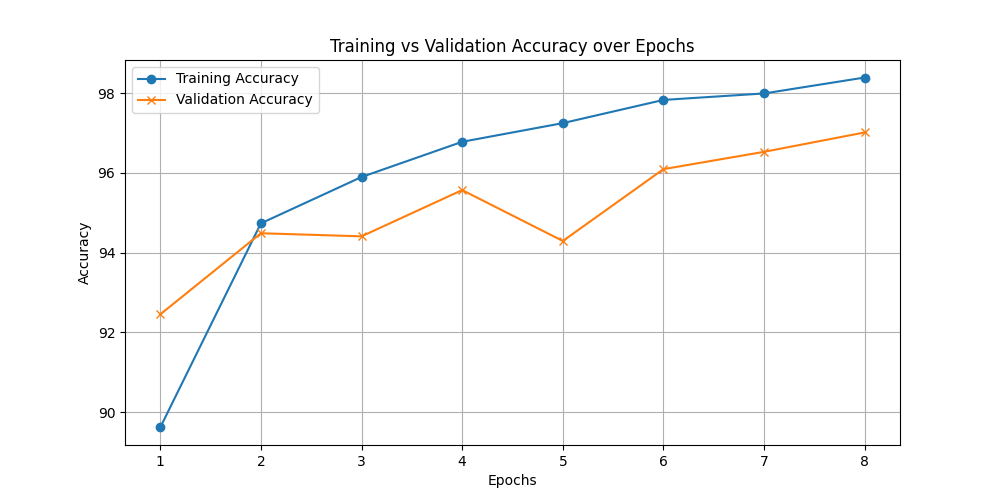
\includegraphics[width=0.75\textwidth]{figures/Resnet18_8_epochs.png}
    \caption{ResNet18 first results.}\label{fig:resNet18first}
\end{figure}

After training with our optimized hyperparameters over more epochs, we already reached an validation accuracy of 99.10\% as can be seen in figure\ref{fig:resNet18opt}

\begin{figure}[ht]
    \centering
    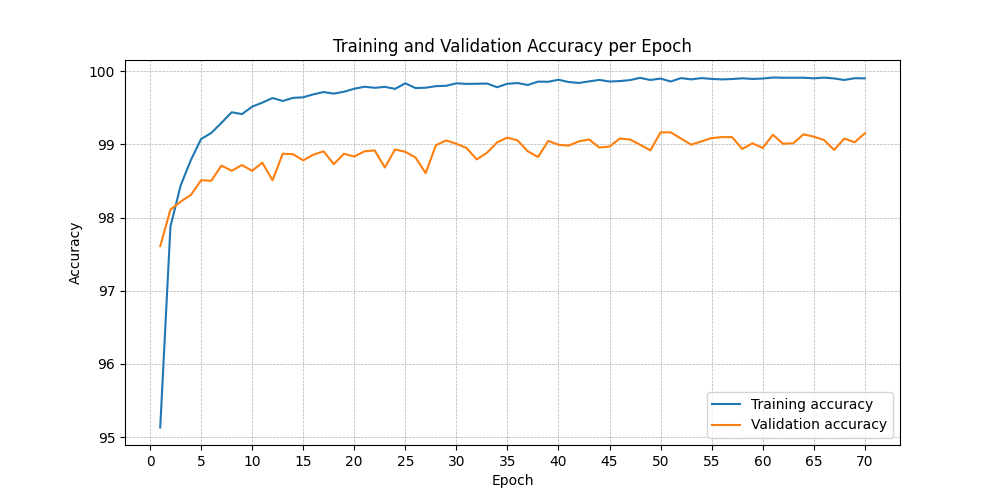
\includegraphics[width=0.75\textwidth]{figures/model_18_v5_accuracy.png}
    \caption{ResNet18 optimised results.}\label{fig:resNet18opt}
\end{figure}

\subsubsubsection{ResNet152:}\label{ResNet152}
Next, we wanted to use deeper models. For this we mostly skipped the models between ResNet18 and ResNet152, as we realized that, while they provided some performance increase, it was too little to focus on them. For the training of ResNet152 we employed the same hyperparameters (table~\ref{tab:hyperparameters}) as for the optimized ResNet18 (figure\ref{fig:resNet18opt}). The results here were a clear but small improvement, as we are already over 99\% accuracy. In figure\ref{fig:resNet152opt}, you can see that our ResNet152 performed at an 99.40\% training accuracy. 

\begin{figure}[ht]
    \centering
    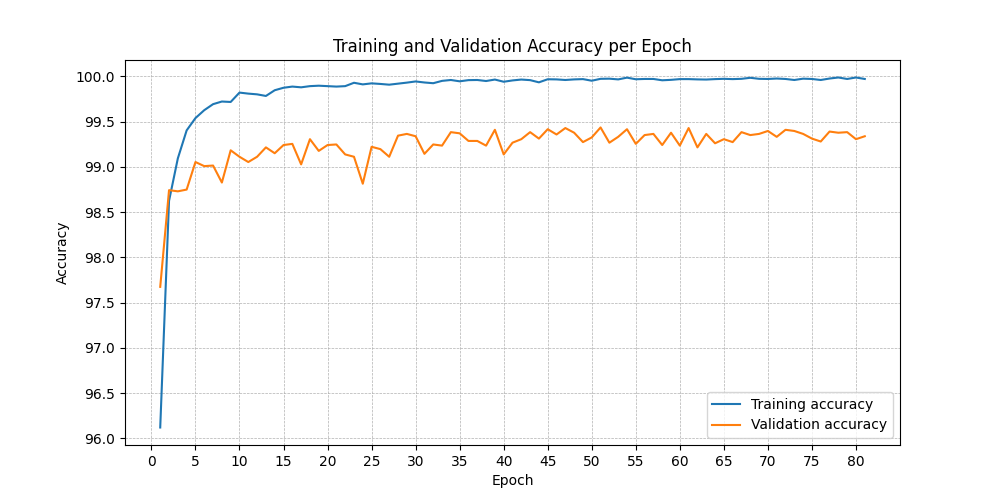
\includegraphics[width=0.75\textwidth]{figures/model_152_v4_accuracy.png}
    \caption{ResNet18 optimised results.}\label{fig:resNet152opt}
\end{figure}

\subsubsubsection{Ensemble Methods:}\label{ensembling}
This is a very complex topic with many different approaches. The core idea is to find a way to combine multiple models together in order to achieve better results. This can be done training one model on the output of multiple different models, train multiple models in a row to improve upon the output of the previous model, and many other ways. As we only wanted to test, if we could get a little bit more performance out of our models, we decided on implementing the most simple version, which just averages the output of different models. Optimally, this would be weighted based on the models strengths and weaknesses. Unfortunately, the strengths and weaknesses for our models were consistent trough all that we trained. All of them struggled with the same classes. Never the less, this still brought some improvements. The performance for these ensemble models we only measured on the test data provided for the Kaggle challenge. There our ensemble of two ResNet152 models, trained with the same parameters outperformed the individual models (each about 99.39\% accuracy) and was our best submission with an accuracy of 99.45\%.  